\section{Description des méthodes de test}
    \subsection{Mobile}
        \subsubsection{Tests unitaires}
        Une panoplies de tests unitaires automatisés ont été effectués. Ces tests résident dans les trois fichiers suivants : «degelClient.test.js», «session.test.js» et «storageHelper.test.js» du dossier «BL/\_\_test\_\_» de notre codebase. Les libraires de tests utilisés sont les suivantes :
        \begin{description}
            \item[Jest expo] Assertions de base, mock de fonctions.
            \item [Jest-fetch-mock] Mock de requêtes HTTP
            \item[Fetch-vcr] Enregistre des requêtes HTTP pour les rejouer lors des tests
            \item[Mock-async-storage] Simule l'environnement de storage du téléphone lorsque les tests tournent sur une machine de développement.
        \end{description}

        Voici une liste des tests unitaires de l'application mobile\footnote{Le titre des tests unitaires est censé décrire ses critères de passation, cependant pour plus de détails concernant les tests des effets de bord («side effects»), il faut se référer au code source des tests de l'application mobile.}.
                
        \begin{table}[hp]
            \centering
            \caption{DEGEL Client}
            \begin{tabular}{P{0.45\textwidth}P{0.45\textwidth}}
\hline
\bf Nom
&
\bf Description
\\
\hline
\hline
\#requestAndSaveAccessTokensWithCode authorized
&
Requête des access tokens réussie
\\
\#requestAndSaveAccessTokensWithCode unauthorized
&
Requête des access tokens non réussie
\\
\#refreshAccessToken
&
Requête des refresh tokens réussie
\\
\#refreshAccessToken unauthorized
&
Requête des refresh tokens non réussie
\\
\#getCurrentUser authorized
&
Obtention de l'utilisateur courant réussie
\\
\#getCurrentUser unauthorized
&
Obtention de l'utilisateur courant non réussie
\\
\#getSettingsStatus authorized
&
Obtention de l'état des paramètres réussie
\\
\#getSettingsStatus unauthorized
&
Obtention de l'état des paramètres non réussie
\\
\#getSettingsStatus unauthorized when id is undefined
&
Obtention de l'état des paramètres non réussie lorsque l'id de l'usager est absent
\\
\#setSettingsStatus unauthorized
&
Requête de changement de paramètres non réussie
\\
\#setSettingsStatus unauthorized when id is undefined
&
Requête de changement de paramètres non réussie lorsque l'id de l'usager est absent
\\
\#setSettingsStatus notification mobile = true
&
Requête de changement de paramètres vers le positif réussie
\\
\#setSettingsStatus notification mobile = false
&
Requête de changement de paramètres vers le négatif réussie
\\
Sends registration token when permission is granted by the user
&
Envoi des tokens de notification réussi
\\
Sends registration token when permission is already granted
&
Envoi des tokens de notification réussi même si déjà envoyés
\\
Does not send registration token when permission is denied by the user
&
Non envoi des tokens de notification lorsque l'usager refuse
\\
registerForPushNotificationsAsync authorized
&
Enregistrement pour des notifications réussi     
\\
\hline
\end{tabular}

            \label{tab.testsDegel}
        \end{table}
        
        \begin{table}[hp]
            \centering
            \caption{Session Tests}
            \begin{tabular}{P{0.3\textwidth}P{0.6\textwidth}}
\hline
\bf Nom
&
\bf Description
\\
\hline
\hline
\#logIn authorized
&
Test d'un login autorisé
\\
\#logIn unauthorized
&
Test d'un login non autorisé
\\
\#logIn unauthorized expired refresh token
&
Test d'un login avec un refresh token expiré
\\
\#logOut remove all stored values
&
Test que le logout supprime toutes les informations de l'utilisateur
\\
\hline
\end{tabular}
            \label{tab.testsSession}
        \end{table}

        \begin{table}[hp]
            \centering
            \caption{Storage Helper}
            \begin{tabular}{P{0.3\textwidth}P{0.6\textwidth}}
\hline
\bf Nom
&
\bf Description
\\
\hline
\hline
\#set save the value when the key does not exists
&
Sauvegarde d'une clé fonctionne lorsqu'elle n'existe psa
\\
\#set override the value when the key exists by removing existing key
&
Sauvegarde d'une clé existante fonctionne
\\
\#set does not save undefined values
&
Ne sauvegarde pas les valeurs non définies
\\
\#set does not save null values
&
Ne sauvegarde pas les valeurs nulles
\\
\#get returns the value
&
Retour de la valeur fonctionne
\\
\#remove remove the value
&
Suppression de la valeur fonctionne
\\
\hline
\end{tabular}
            \label{tab.testsStorage}
        \end{table}
                
        \subsubsection{Tests d'intégration}
        Voici les scénarios de tests d'intégrations mobile. Ces tests d'intégrations sont fait et vérifiés manuellement :

        \begin{table}[hp]
            \centering
            \caption{Tests d'intégration sur mobile}
            \begin{tabular}{P{0.3\textwidth}P{0.6\textwidth}}
\hline
\bf Scénario
&
\bf Résultat escompté
\\
\hline
\hline
Un usager ouvre l'application pour la première fois
&
Il observe une page qui l'invite à se connecter
\\
L'usager appui sur le bouton de connexion
&
L'usager est redirigé vers CAS
\\
L'usager entre des informations sur CAS puis se connecter
&
L'usager est redirigé vers l'application
\\
L'usager appui sur le bouton de retour dans la vue CAS
&
L'usager est redirigé vers la page précédente
\\
L'usager appui sur le bouton X de la vue CAS
&
L'usager revient à la page d'accueil
\\
L'usager consulte son horaire une fois connecté
&
Les événements de son calendrier horarius s'affichent
\\
L'usager se déplace de journée
&
L'usager peut voir les événements de plusieurs semaines qui sont chargés dynamiquement
\\
L'usager appui sur le bouton de retour à la journée présente
&
L'usager retourne à la journée présente
\\
L'usager appui sur le bouton des paramètres
&
L'usager se voit rediriger vers la vue paramètre
\\
L'usager se désinscrit des notifications
&
L'usager ne reçoit plus de notifications
\\
L'usager s'inscrit aux notifications
&
L'usager peut recevoir des notifications
\\
L'usager est inscrit aux notifications
&
L'usager reçoit des notifications lors d'un changement d'horaire
\\
L'usager se déconnecte
&
Toute les informations sauvegardés de l'usager sont supprimés du téléphone
\\
\hline
\end{tabular}
            \label{tab.testsIntegrationMobile}
        \end{table}
                
    \subsection{Backend}

        \subsubsection{Tests unitaires}
        Plusieurs frameworks tel JUnit et mockk (équivalent Kotlin de Mockito) ont été utilisés du côté backend pour effectuer une série de tests unitaires. Ceux-ci reposent sur l'injection de dépendances par souci de praticité ce qui permet de ne tester qu'un module à la fois. Comme la logique d'affaire se retrouve principalement dans les services et les helpers, ce sont eux qui ont été principalement testés. Les tests se trouvent tous dans le dossier  src/tests/kotlin/ca/usherbrooke.degel.

        \begin{table}[hp]
            \centering
            \caption{Tests backend}
            % One must insert an empty line between '\\' and '[', otherwise TeX is looking for a vertical space value between the brackets
\begin{tabular}{P{0.3\textwidth}P{0.6\textwidth}}
\hline
\bf Nom
&
\bf Description
\\
\hline
\hline%

[Helper] Test diff calendars
&
Test du helper de différences de calendriers (ajout, suppression, modification)
\\%

[Helper] Test same events
&
Test du helper de différences d'événements (dates, local, professeur)
\\%

[Settings] Get user settings
&
Test le fetch des préférences de l'utilisateur
\\%

[Settings] When no settings get default settings
&
Test que les préférences par défaut sont retournées pour un nouvel utilisateur
\\%

[Settings] If no settings insert them
&
Test que les nouvelles préférences de l'utilisateur sont enregistrées
\\%

[Settings] If settings present update them
&
Test que les préférences de l'utilisateur sont mises à jour
\\%

[Calendrier] If no calendar insert it
&
Test l'insertion de l'entité calendrier si non présent
\\%

[Calendrier] If calendar present update the key
&
Test la mise à jour de la clé horarius
\\%

[Calendrier] If no calendar throw
&
Test l'exception si le système n'a pas de calendar lorsque demandé
\\%

[Calendrier] If empty calendar key throw
&
Test l'exception si le système à une clé horarius vide
\\%

[Calendrier] If invalid key throw
&
Test l'exception si le système détecte une clé invalide
\\%

[Calendrier] Get user calendar
&
Test l'utilisation normale du client horarius
\\%

[Calendrier] If fetching error throw
&
Test l'exception si horarius retourne une erreur
\\%

[Calendrier] Get stored calendar
&
Test l'extraction du calendrier ical enregistré dans la BD
\\%

[Calendrier] Update calendar for user
&
Test l'update du calendrier ical dans la BD
\\%

[Calendrier] Cannot insert invalid calendar key
&
Test l'exception si l'utilisateur tente d'insérer une clé invalide
\\%

[Notifications] When new token add token
&
Test d'ajout d'un nouveau token Expo
\\%

[Notifications] When duplicate token delete old token and then add new token
&
Test le remplacement d'un Token en cas de duplicata
\\%

[Général] Test context load
&
Test que l'application peut démarrer (long test)
\\
\hline
\end{tabular}
            \label{tab.testsBackend}
        \end{table}
        
        \subsubsection{Tests d'intégration}
        Un interface swagger a été installée sur notre backend. Celle-ci permet facilement d'effectuer des tests d'intégrations pour tout nos end-points. Swagger est une belle interface graphique qui permet de faire des requêtes HTTP autorisés à des endpoints en injectant les bonnes données. Il reste ensuite à observer le résultat pour savoir si la fonctionnalité marche ou non. Les tests d'intégrations du backend ont été effectués manuellement.
        
        \begin{figure}[hp] \centering
            \centering
            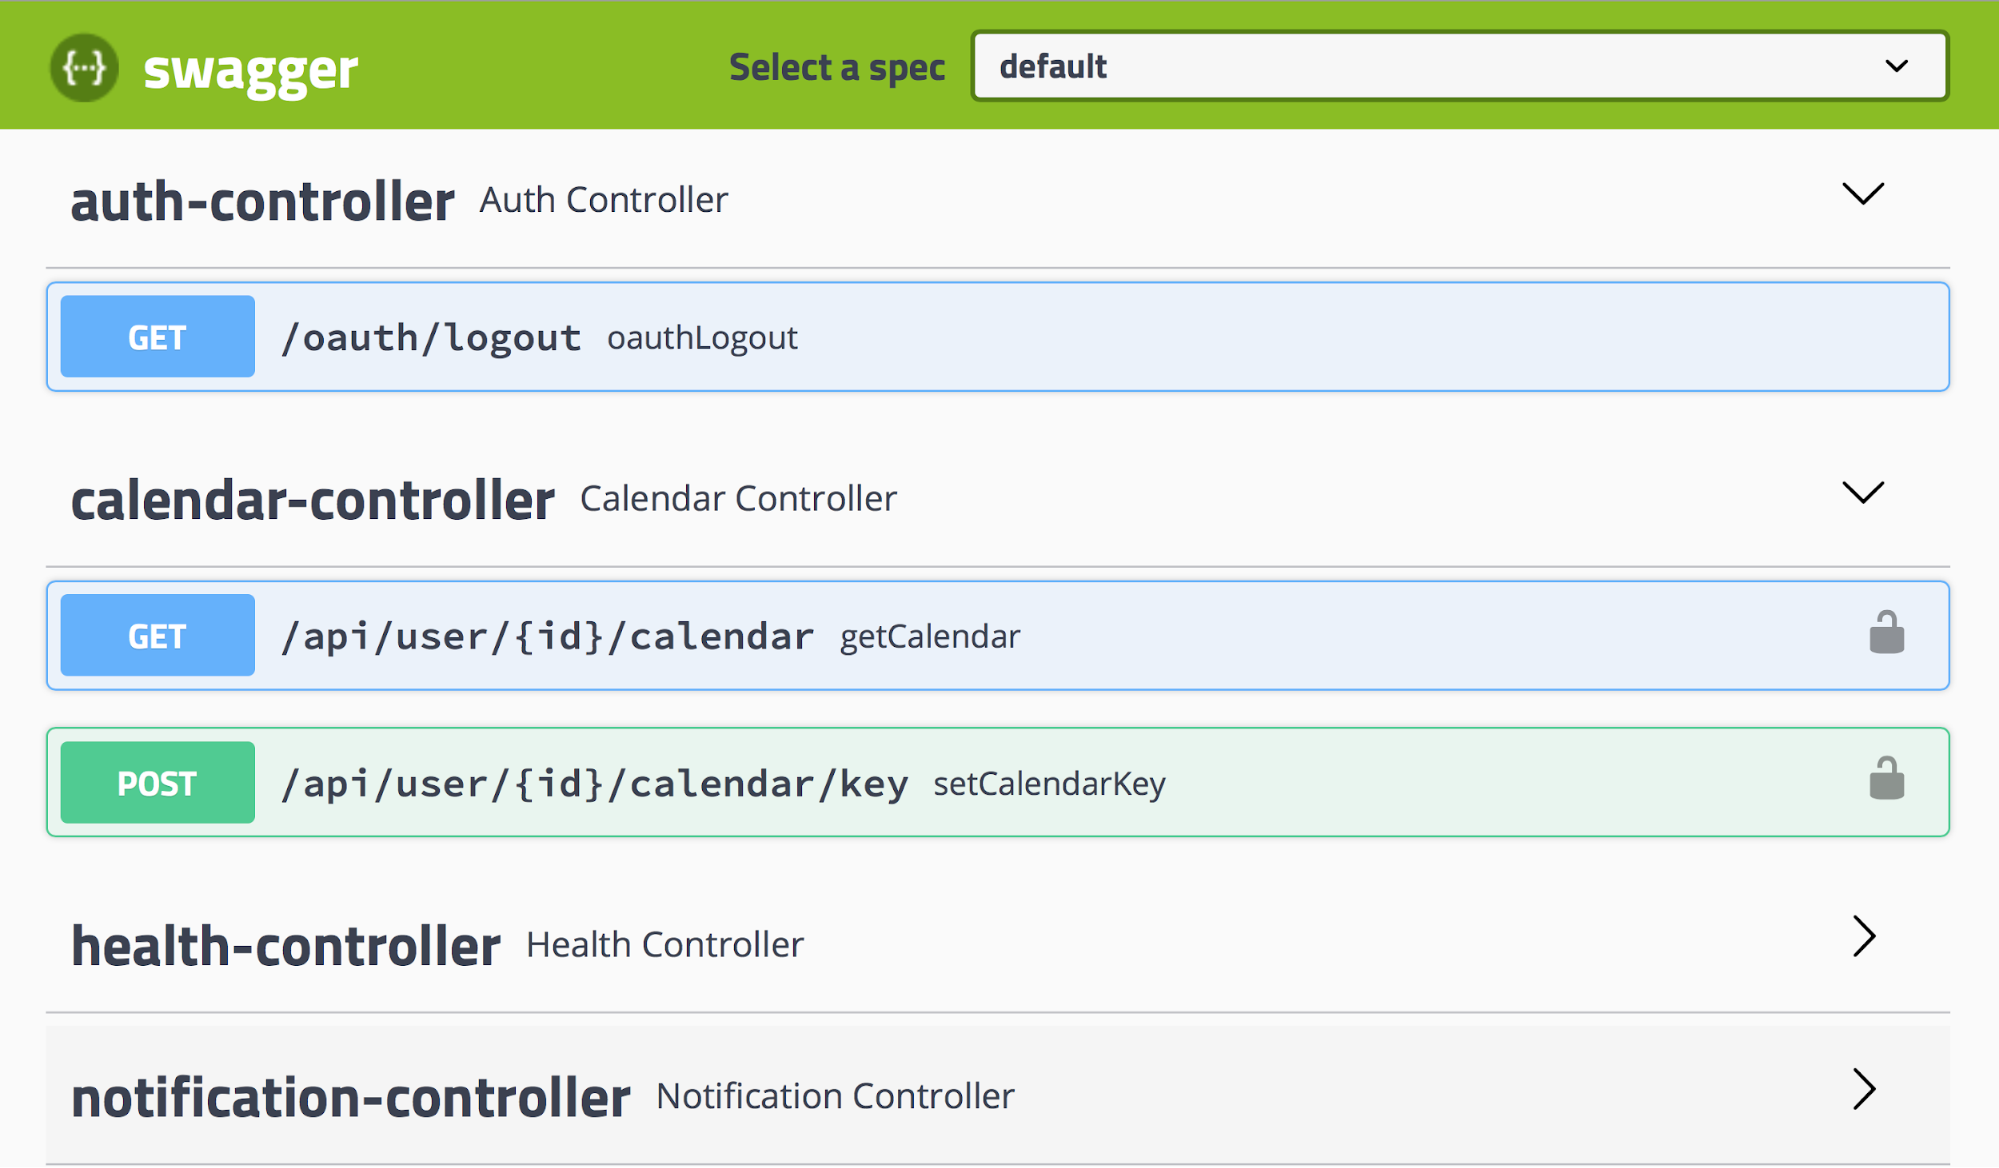
\includegraphics[width=\textwidth]{Figures/swagger}
            \caption{Interface swagger du backend}
            \label{fig.swagger}
        \end{figure}
        
                